\documentclass{beamer}
\usepackage{tcolorbox}

%\beamerdefaultoverlayspecification{<+->}
\newcommand{\data}{\mathcal{D}}

\DeclareMathOperator*{\argmax}{arg\,max}

\newcommand\Item[1][]{%
	\ifx\relax#1\relax  \item \else \item[#1] \fi
	\abovedisplayskip=0pt\abovedisplayshortskip=0pt~\vspace*{-\baselineskip}}
\usepackage{amsmath}
\usepackage{amssymb}
\usepackage{subfig}


\usetheme{metropolis}           % Use metropolis theme


\title{Bayesian Machine Learning, MLE, MAP - I}
\date{\today}
\author{Nipun Batra}
\institute{IIT Gandhinagar}

\begin{document}
\maketitle

\begin{frame}{Bayesian Machine Learning}
\begin{itemize}[<+->]
\item Allows us to incorporate prior knowledge into the model, \emph{irrespective} of what the data has to say. 
\item Particularly useful when we do not have a large amount of data - use what \emph{we} know about the model than depend on the data.
\item Also allows us to predict with confidence quantified typically using variance.
\end{itemize}
\end{frame}

% \begin{frame}{An example - Coin Flip}
% \begin{itemize}
% \item Suppose we want to learn the probability that head shows up when a coin is tossed. This probability is a \emph{parameter} to be learnt.
% \item 
% \item An example: Time-series meteorological data - temporal patterns in temperature.
% \item Particularly useful when we do not have a large amount of data. 
% \end{itemize}
% \end{frame}


 
 
  
  
% \section{Linear Regression}

% \begin{frame}{Bayes Rule in Continuous Sense}
% \begin{itemize}
	
	
% 	\item $P(A | B) = \frac{P(B|A)P(A)}{P(B)}$, where $A$ and $B$ are random variables.
% 	\item $P(X)$ is the PDF of $X$ where $X$ is a continuous random variable.
% 	\item In the Bayesian setting, we assume that the parameters of our machine learning come from a distribution. We also assume that the data was typically generated from some probability distribution.
	
% % 	\item Examples of linear systems:
% % 	\begin{itemize}
% % 		\item $F=ma$
% % 		\item $v=u+at$
% % 	\end{itemize}
	
% \end{itemize}
% \end{frame}

{
	\setbeamercolor{background canvas}{bg=}
	
\includepdf[page=1-]{bayes.pdf}
}

\begin{frame}{Bayes Rule}
\begin{itemize}[<+->]
	\item Bayes Rule: $P(A | B) = \frac{P(B|A)P(A)}{P(B)}$.
	\item Example:  You tested positive for a disease. But, the test is only 99\% accurate.
	\item $P(Test = +ve | Disease = True) = 0.99$
	 \item $P(Test = -ve | Disease = False) = 0.99$
	 \item Also, the disease is a rare one. Only one in 10,000 has it.
	 \item Given the result of test is positive, what is the probability that someone has the disease?
\end{itemize}
\end{frame}

\begin{frame}{Bayes Rule}
\begin{itemize}
	\item $P(T|D)$ = 0.99
	\item $P(\bar{T}|\bar{D})$ = 0.99
	\item $P(T|\bar{D})$ = 0.01
	\item $P(\bar{T}|D)$ = 0.01
	\item $P(D)$ =$ 10^{-4}$
	\item $P(\bar{D})$ =$ 1 - 10^{-4}$
\end{itemize}

Given the above, calculate $P(D|T)$. 
\end{frame}

\begin{frame}{Problem}
\begin{align}
\label{eqn*:eqlabel}
\begin{split}
P(D|T) &= \frac{P(T|D)P(D)}{P(T)}
\end{split}
\end{align}



\end{frame}

\begin{frame}{Problem}
\begin{align}
\label{eqn*:eqlabel}
\begin{split}
P(D|T) &= \frac{P(T|D)P(D)}{P(T)}\\
&=\frac{P(T|D)P(D)}{P(T|D)P(D) + P(T|\bar{D})P(\bar{D})}
\end{split}
\end{align}

$$
=\frac{(.99)\left(10^{-4}\right)}{(.99)\left(10^{-4}\right)+(.01)\left(1-10^{-4}\right)}
$$
\end{frame}

\begin{frame}{Problem}
\begin{align}
\label{eqn*:eqlabel}
\begin{split}
P(D|T) &= \frac{P(T|D)P(D)}{P(T)}\\
&=\frac{P(T|D)P(D)}{P(T|D)P(D) + P(T|\bar{D})P(\bar{D})}
\end{split}
\end{align}

$$
=\frac{(.99)\left(10^{-4}\right)}{(.99)\left(10^{-4}\right)+(.01)\left(1-10^{-4}\right) } = 0.09 << 0.99
$$

\end{frame}

\begin{frame}{Bayes Rule}
\begin{itemize}[<+->]

	\item Notation: Let $\theta$ denote the parameters of the model and let $\mathcal{D}$ denote observed data. From Bayes Rule, we have 
	\begin{equation*}
	    P(\theta | \mathcal{D}) = \frac{ P(\mathcal{D}|\theta)P(\theta) }{P(\mathcal{D})}
	\end{equation*}
	\item In the above equation $P(\theta | \mathcal{D})$ is called the posterior, $P(\mathcal{D}|\theta)$ is called the likelihood, $P(\theta)$ is called the prior and $P(\mathcal{D})$ is called the evidence.
% 	\item Examples of linear systems:
% 	\begin{itemize}
% 		\item $F=ma$
% 		\item $v=u+at$
% 	\end{itemize}
	
\end{itemize}
\end{frame}
\begin{frame}{Likelihood, Prior and Posterior}
\begin{itemize}[<+->]
	
	\item Likelihood $P(\mathcal{D}|\theta)$ quantifies how the current model parameters describe the data. It is a function of $\theta$.  Higher the value of $P(\mathcal{D}|\theta)$, the better the model describes the data.
	\item Prior $P(\theta)$ is the knowledge we incorporate into the model, \emph{irrespective} of what the data has to say. As an example, if we have $n$ model parameters, $\theta \stackrel{}{\sim} \mathcal{N}(0,I_n)$ could be the knowledge we are incorporating into the model.
	\item Posterior $P(\theta | \mathcal{D})$ is the probability that we assign to the parameters after observing the data. Posterior takes into account prior knowledge unlike likelihood.
	\item Posterior $\propto$ Likelihood $\times$ Prior
\end{itemize}
\end{frame}


\begin{frame}{Bayesian Learning is well suited for online learning}
\begin{itemize}[<+->]
\item In online learning, data points arrive one by one. We can index this using timestamps. So we have one data point for each timestamp.
\item Initially no data: We only have $P(\theta)$, which is prior knowledge which we have about the model parameters, \emph{without} observing any data.
\item Suppose we observe $\mathcal{D}_1$ at timestamp 1. Now we have new information. This knowledge is encoded as $P(\theta | \mathcal{D}_1)$. 
\item Now, $\mathcal{D}_2$ arrives at timestamp 2. Now we have $P(\theta | \mathcal{D}_1)$, acting as the prior knowledge before we observe $\mathcal{D}_2$.
\item Similarly, for timestamp $n$, we will have $P(\theta | \mathcal{D}_1, \mathcal{D}_2, \mathcal{D}_3, \dots \mathcal{D}_{n-1})$ acting as the prior knowledge before we observe $\mathcal{D}_n$.
\end{itemize}
\end{frame}

\begin{frame}{Bayesian Learning is well suited for online learning}
\begin{figure}[htp]
    \centering
    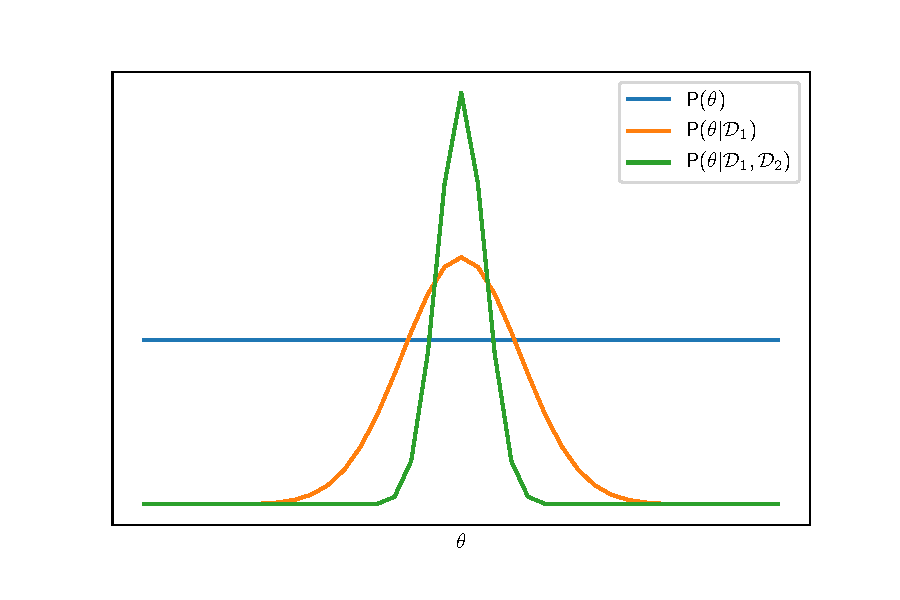
\includegraphics[width=9cm]{plots/online.pdf}
    \caption{Online Learning: Variation of Prior as more data points arrive.}
    \label{fig:online}
\end{figure}

\end{frame}

\begin{frame}{Aside on Bernoulli Likelihood}
\begin{itemize}[<+->]
	\item Assume you have a coin and flip it ten times and get (H, H, T, T, T, H, H, T, T, T).
	\item What is p(H)?
	\item We might think it to be: 4/10 = 0.4. But why?
	\item Answer 1: Probability defined as a measure of long running frequencies
	\item Answer 2: What is likelihood of seeing the above sequence when the p(Head)=$\theta$?
	\item Idea find MLE estimate for $\theta$
\end{itemize}

\end{frame}

\begin{frame}{Aside on Bernoulli Likelihood}
\begin{itemize}[<+->]
\item $p(H) = \theta$ and $p(T) = 1 - \theta$
\item What is the PMF for first observation $P(D_1 = x|\theta)$, where x = 0 for Tails and x = 1 for Heads?
\item $P(D_1 = x|\theta) = \theta^x(1-\theta)^{(1-x)}$
\item Verify the above: if x = 0 (Tails), $P(D_1 = x|\theta) = 1 - \theta$ and if x = 1 (Heads), $P(D_1 = x|\theta)  = \theta$
\item What is $P(D_1, D_2, ..., D_n|\theta)$?
\item $P(D_1, D_2, ..., D_n|\theta) = P(D_1\theta)P(D_2|\theta)...P(D_n|\theta)$
\item $P(D_1, D_2, ..., D_n|\theta) =\theta^{n_h}(1-\theta)^{n_t}$
\item Log-likelihood = $\mathcal{LL}(\theta) = n_h\log(\theta) + n_t\log(1-\theta)$
\item $\frac{\partial \mathcal{LL}(\theta)}{\partial \theta} = 0 \implies \frac{n_h}{\theta} + \frac{n_t}{1-\theta} = 0 \implies \theta_{MLE} = \frac{n_h}{n_h + n_t}$

\end{itemize}

\end{frame}





% \begin{frame}{Bayes Rule for Machine Learning}
% \begin{itemize}


%     \item $P(A|B)P(B) = P(B|A)P(A)$
%     \item Let us consider for a machine learning problem:
%     \begin{itemize}
%     	\item A = Parameters ($\theta$)
%     	\item B = Data ($\mathcal{D}$)
%     \end{itemize}
% \item We can rewrite the Bayes rule as:
% \begin{itemize}
% 	\item $P(\theta|\mathcal{D}) = \frac{P(\mathcal{D}|\theta)P(\theta)}{P(\mathcal{D})}$
% 	\item Posterior: 
% 	\item Prior:
% 	\item Likelihood
% 	\item 
% \end{itemize}
% \end{itemize}
% \end{frame}

% \begin{frame}{Likelihood}
% \begin{itemize}
% 	\item Likelihood is a function of $\theta$
% 	\item Given a coin flip and 5 H and 1 T, what is more likely: P(H) = 0.5 or P(H) = 0.9
% \end{itemize}
% \end{frame}

% \begin{frame}{Bayesian Learning is well suited for online settings}
% content...
% \end{frame}

%\begin{frame}{Coin flipping}
%\begin{itemize}
%	\item Assume we do a coin flip multiple times and we get the following observation: \{H, H, H, H, H, H, T, T, T, T\}: 6 Heads and 4 Tails
%	\item  What is $P(Head)$?
%	\item Is your answer: 6/10. Why?
%\end{itemize}
%
%\end{frame}

%\begin{frame}{Coin flipping: Maximum Likelihood Estimate (MLE)}
%\begin{itemize}
%	\item We have $\mathcal{D} = \{\data_1, \data_2, ...\data_{N}\}$ for $N$ observations where each $\mathcal{D}_i \in \{H, T\}$
%	\item Assume we have $n_H$ heads and $n_T$ tails, $n_H + n_T = N$
%	\item Let us have $P(H) = \theta, P(T) = 1-\theta$
%	\item We have Likelihood, $L(\theta) = P(\mathcal{D}|\theta) = P(\data_1, \data_2, ..., \data_N|\theta)$
%	\item Since observations are i.i.d., $L(\theta) = P(\data_1|\theta).P(\data_2|\theta) ... P(\data_N|\theta)$
%\end{itemize}
%
%\end{frame}


%\begin{frame}{Coin flipping: Maximum Likelihood Estimate (MLE)}
%\begin{itemize}
%	\item  
%\begin{align*}  
%P(\data_i|\theta) =  \left
%\{\begin{array}{lr} \theta, & \text{for~} \data_i =H \\
%1-\theta, & \text{for~} \data_i = T
%\end{array}\right.\
%\end{align*}  
%\item Thus, $L(\theta) = \theta^{n_H}\times (1-\theta)^{n_T}$
%\item Log-Likelihood, $LL(\theta) = n_Hlog\theta + (n_T)(log(1-\theta))$
%\item $\frac{\partial LL(\theta)}{\partial \theta} = \frac{n_H}{\theta} - \frac{n_T}{1-\theta}$
%\item  For optima, set derivative of LL to zero.
%
%\item 	$\frac{n_H}{\theta} - \frac{n_T}{1-\theta} = 0 $
%\end{itemize}
%% \begin{tcolorbox}
%	\begin{align*}
%	 \theta = \frac{n_H}{n_H + n_T}
%	\end{align*}

% \end{tcolorbox}


%\end{frame}

\begin{frame}{}
Question: Is this maxima or minima?
\pause \begin{align*}
\frac{\partial^2 LL(\theta)}{\partial \theta^2} = \frac{-n_H}{\theta^2} + \frac{-n_T}{(1-\theta)^2} \in \mathbb R_-
\end{align*}
Thus, the solution is a maxima.

\pause Any issues with maximum likelihood estimate or MLE?



\end{frame}

\begin{frame}{Maximum A Posteriori estimate (MAP)}
\begin{itemize}


\item \textbf{MLE does not handle prior knowledge}: What if we know that our coin is biased towards head?
\item \textbf{MLE can overfit}: What is the probability of heads when we have observed 6 heads and 0 tails?
\end{itemize}

\end{frame}


\begin{frame}{Maximum A Posteriori estimate (MAP)}
Goal: Maximize the Posterior
% \begin{tcolorbox}
	\begin{align}
\hat{\theta}_{MAP} = \argmax_\theta P(\theta|\data)\\
\hat{\theta}_{MAP}= \argmax_\theta P(\data|\theta)P(\theta)
\end{align}
% \end{tcolorbox}

\end{frame}
%
%\begin{frame}{Prior distributions}
%\begin{figure}
%    \centering
%    \subfloat{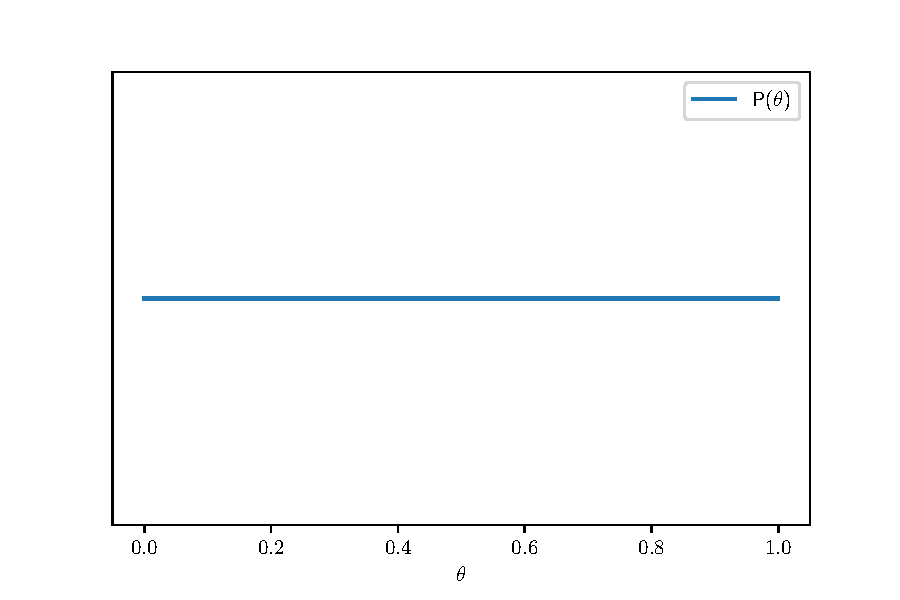
\includegraphics[width=4.5cm]{plots/uniformprior.pdf} }
%    \qquad
%    \subfloat{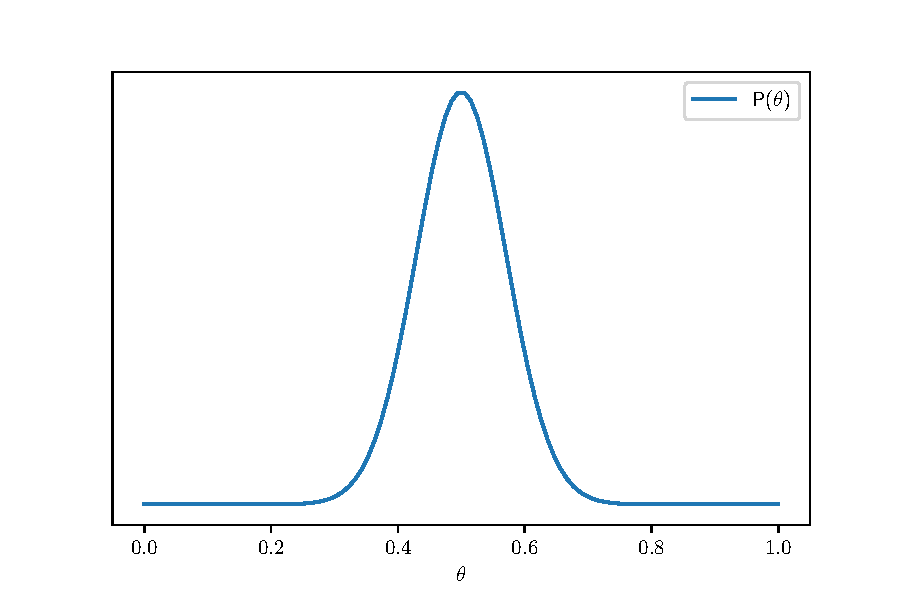
\includegraphics[width=4.5cm]{plots/nonuniformprior.pdf} }
%    \caption{Uniform and Non Uniform Prior.}
%    \label{fig:example}
%\end{figure}
%\end{frame}
%
%
%\begin{frame}{Beta Distribution}
%\begin{itemize}
%    \item It is a continuous probability distribution defined on $[0, 1]$, which has two parameters $a$ and $b$.
%
%    \item $Beta(\theta | a, b) = \frac{\Gamma(a + b)}{\Gamma(a)\Gamma(b)}\theta^{a-1}(1 - \theta)^{b - 1}$. Note the similarity with the binomial distribution.
%    \item $\Gamma(n) = (n - 1)!$ when $n$
% is a natural number.
% \item $\Gamma(z) = \int_0^\infty x^{z-1}e^{-x}dx$
%
% \end{itemize}
%\end{frame}
%
%\begin{frame}{Beta Distribution Examples}
%\begin{itemize}
% \item $Beta(\theta | 1, 1) = \frac{\Gamma(2)}{\Gamma(1)\Gamma(1)}\theta^{1 - 1}(1 - \theta)^{1 - 1}$ = 1. This is the uniform distribution on [0,1].
% \item  $Beta(\theta | 2, 2) = \frac{\Gamma(4)}{\Gamma(2)\Gamma(2)}\theta(1 - \theta) = 6\theta(1 - \theta)$. 
% 
% \begin{figure}[htp]
%    \centering
%    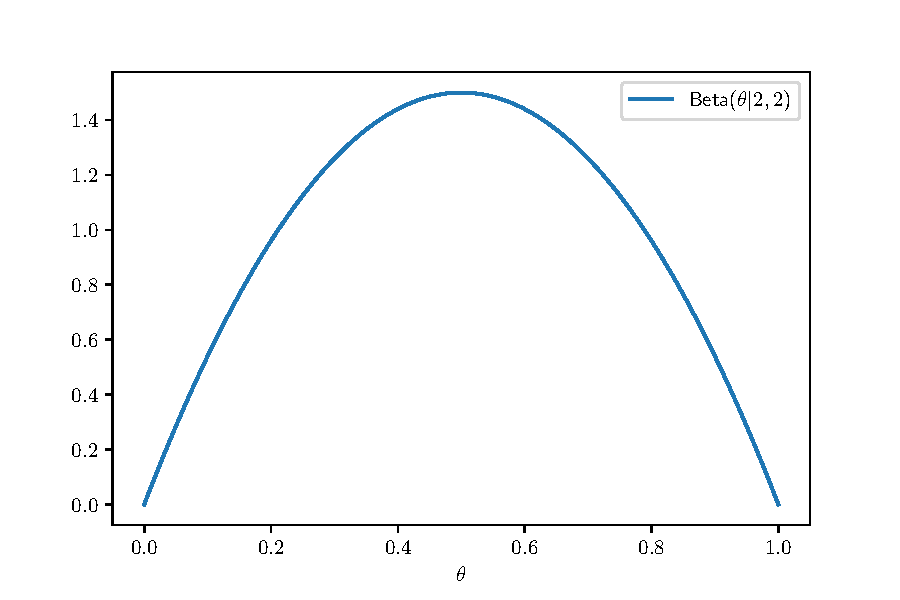
\includegraphics[width=5cm]{plots/beta22.pdf}
%    \caption{Beta($\theta|2,2)$}
%    \label{fig:beta22}
%\end{figure}
%\item Note: $Beta(\theta | a, 1)$ indicates higher probability of heads than tails.
%
% \end{itemize}
%\end{frame}
%
%\begin{frame}{Coin toss: MAP estimate}
%\begin{itemize}
%    
%\item $\mathcal{D} = n_H, n_T$
%\item $P(\theta) = Beta(\theta | a, b) = \frac{\Gamma(a + b)}{\Gamma(a)\Gamma(b)}\theta^{a - 1}(1 - \theta^{b - 1})$.
%\item $\hat{\theta}_{MAP} =\argmax_\theta P(\mathcal{D}|\theta)P(\theta)$ 
%\item   $\implies \hat{\theta}_{MAP} =  \argmax_\theta \theta^{n_H}(1 - \theta)^{n_T}\theta^{a - 1}(1 - \theta)^{b -1} \times k$
%\item Equivalently, $\hat{\theta}_{MAP}$ = $\argmax_\theta \theta^{n_H + a - 1}(1 - \theta)^{n_T + b - 1}$
%\item $\therefore \hat{\theta}_{MAP} = \frac{n_H + a - 1}{n_H + n_T + a + b - 2}$
%\end{itemize}
%\end{frame}
%
%\begin{frame}{Conjugate Prior}
%	\begin{equation*}
%	    P(\theta | \mathcal{D}) = \frac{ P(\mathcal{D}|\theta)P(\theta) }{P(\mathcal{D})}
%	\end{equation*}
%\begin{itemize}
%    \item $P(\theta)$ is conjugate to $P(\mathcal{D}|\theta)$ if $P(\theta | \mathcal{D})$ and $P(\theta)$ are from the same distribution family.
%    \item Example: Bernoulli likelihood has gamma as conjugate.
%\end{itemize}
%\end{frame}
%
%\begin{frame}{Relationship between MLE and MAP}
%\begin{itemize}
%    \item When is $\hat{\theta}_{MAP}$ = $\hat{\theta}_{MLE}$?
%    \item Answer: When prior $P(\theta)$ is uniform, maximizing the likelihood is the same as maximizing the posterior distribution.
%\end{itemize} 
%\end{frame}
%
%
%% \begin{frame}{Linear Regression: MLE}
%% We previously saw 
%% \begin{tcolorbox}
%% \begin{align*}
%% \hat{\theta}_{least-square} = \argmin_\theta \epsilon^T\epsilon = \argmin_\theta (y-X\theta)^T(y-X\theta)
%% \end{align*}
%% \end{tcolorbox}
%
%% \end{frame}
\end{document}

